\chapter{Design of the Evaluation Scheme}
\label{chap:System}

This chapter walks through the steps taken in order to build our evaluation system and describes its keys components in detail.

%Maybe should be moved to introduction?
\section{Design Criteria}

Since outdoor AR applications are the focus of this research, we have designed our evaluation model within this framework. Moreover, all the proposed evaluation
metrics are measured based on the relevant factors described earlier in the previous chapters.

%%%
%In these models, a pixel is considered as an \textit{outlier} if the error between the ground truth disparity and the disparity found by the solution is more than 
%a specified pixel threshold in the system, such as 2 or 3 pixels.
%They also provide separate masks for depth discontinuities and occluded regions, in addition to evaluating the whole image.
%%%

%However, both models take a general approach towards evaluating stereo algorithms; that is they have not been designed with an eye to the particular target 
%application.


%In other words, they mainly focus on the fundamental aspects of designing a stereo algorithm as a solution per se to \textit{efficiently}
%find the \textit{best matches} of corresponding pixels in stereo pairs. 
%This perspective may raise some questions for a punctilious researcher, such as:

%\begin{enumerate}
%\item What actually is an \textit{efficient} solution and on what basis is this \textit{efficiency} defined?
%\item What is a \textit{best match} of corresponding pixels and how can it be defined?
%\end{enumerate}


%In fact, these questions have compelled us to study the evaluation of the stereo matching solutions from a different point of view.
%In this design, we take steps towards an evaluation design which is based on the potential applications of stereo methods.
%This enables us to better define and adjust the criteria for \textit{efficiency} and 
%\textit{the best correspondence matches} while doing the evaluation.
%Since AR has attracted more attention in the past few years, 
%the evaluation scheme proposed in this study is designed based on outdoor AR applications which take advantage of
%stereo vision techniques to obtain a depth map of the surrounding environment. This map will then be used to
%integrate virtual objects in the scene that respect the occlusion property and the depth of the real objects in the scene. 
%In other words, the motivation of this research is to study the possibility and usability of integrating stereo vision techniques in an AR system, while considering the most
%important constraints that AR systems normally encounter \cite{liv05}.
%Move to Introduction Chapter

\section{A Comprehensive Evaluation Scheme}

In an augmented reality system, there are certain factors that would affect the functionality and effectiveness of the system \cite{liv05,kru10} and, therefore, 
should be carefully considered when designing and evaluating the system.
These factors, which correspond to different components of an AR system, are related to the surrounding 
environment, human factors in AR, or technology and hardware constraints.
Figure \ref{fig:AR} illustrates a high level architecture of our ultimate AR system with its key components.

\begin{figure}[H]
\centering
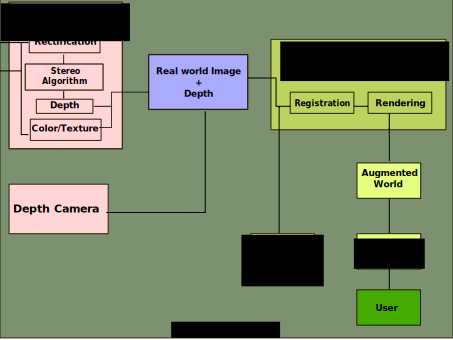
\includegraphics[scale=0.75]{AR}
\caption{High-level architecture of an AR system}
\label{fig:AR}
\end{figure} 

%Concentrating on the requirements of providing a real-time interaction between an AR system and the users, along with
%certain human factors that would affect the functionality of the system,
%has revealed the necessity of involving them in the evaluation of the stereo correspondence methods. Therefore, in order to 
%determine whether a stereo correspondence algorithm can meet the requirements of an AR application, we need an evaluation scheme which can properly assess 
%the \textit{efficiency} of the algorithm and the accuracy of its disparity results based on specific human factors in binocular vision and augmented reality.
%These factors are in fact the concepts related to real-time responsiveness of an AR system mentioned in \ref{chap:Introduction}, and binocular vision, stereopsis, human perception of depth, 
%and stereoacuity as thoroughly described in \ref{chap:BinocularVision}.

%In other words, we have proposed and desgined an evaluation scheme that studies some of the most important aspects of a system that consists of both
%AR and stereo vision components, thus enabling the designers to better evaluate the stereo correspondence solutions that will be intergrated 
%in the system.

In our design, unlike the Middlebury or Kitti benchmarks, we label a pixel in the disparity results as an \textit{outlier} if the angular
measurement, that is in form of stereoacuity, corresponding to the depth error between the ground truth and the estimated depth value by the 
algorithm is more than the minimum perceptible stereoacuities
for the human visual system as determined
by standard stereo tests \cite{binr83,garn06}. 
Moreover, we use the average stereoacuity for different age groups \cite{garn06} in our design to evaluate the performance of the algorithm for users 
at different ages; this makes the evaluation results more reliable and applicable to practical applications of AR.
In order to evaluate the efficiency of an algorithm and investigate whether it meets the requirements for being part of a real-time AR application, 
we have integrated a module in the evaluation process that reports on the average execution time of the algorithm for the input data.
The average outliers based on the specified stereoacuity thresholds and the average disparity error are also estimated during the evaluation process.

In addition, our model employs a particular approach which can be of specific value to practical AR applications. In this approach, we suggest that
it is prudent to focus the evaluation process on the particular regions of the disparity map rather than the whole image. The main hypothesis
is that salient edges caused by depth discontinuities, which also represent object boundaries and occlusion, are important depth cues for the human
visual system to better perceive the location of different objects in the 3D environment \cite{sze11}.
Based on this hypothesis, we argue that more accurate depth results in these regions allows for a higher quality combination of the depth map of the real world with the 
virtual depth of the synthetic objects that are part of the AR scene.
%In other words, in our model we have i
%exclusively applying and studying the evaluation process on those regions in the disparity map rather than the whole image.

\section{Design Overview}

Our evaluation model consists of the following key components:

\begin{itemize}
\item Stereo pairs, calibration data, and ground truth disparity (occluded or non-occluded) as inputs
\item Edge region masks generated from the ground truth disparity maps
\item Masked ground truth disparity
\item Full and masked disparity maps generated by the stereo algorithm 
\item Main evaluation module
\item Evaluation metrics output as data files and plots
\end{itemize}

It should be noted that some of these components, such as the masked ground truth, or the masked disparity maps 
can be optionally built during the process depending on the specific parameters set at the run time of each step. Figure \ref{fig:higharch} shows the high level block diagram of our design.

\begin{figure}[H]
\centering
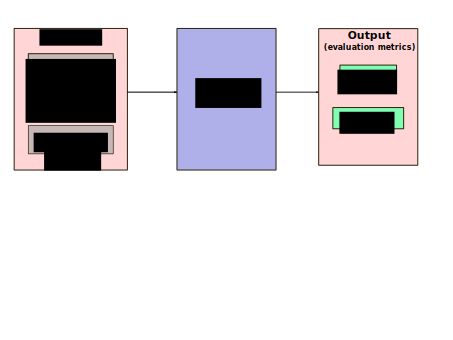
\includegraphics{EvalSyshigh}
\caption{High-level block diagram of the evaluation system}
\label{fig:higharch}
\end{figure} 
\noindent
A lower level architecture of our evaluation system is shown in Figure \ref{fig:lowarch}. This figure illustrates the 
sequence of the operations during the whole process. 

As can be seen in Figure \ref{fig:lowarch}, first the input data consisting of the stereo images, the ground truth disparity, and 
the calibration data are passed to the system.
Afterwards, the specified masks are created using a \textit{Canny} edge detector and a \textit{Dilation} operation with the appropriate parameters 
selected separately for each image.
After the corresponding disparity maps have been generated by the stereo algorithm and stored on the disk, 
they are passed to the evaluation module with the specified arguments.
Finally, the evaluation metrics are estimated and output as data files and plots to facilitate the evaluation of the stereo algorithm in the application
of interest, outdoor AR systems.

\begin{figure}[H]
\centering
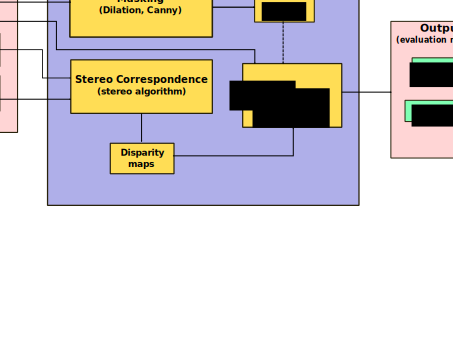
\includegraphics{EvalSyslow}
\caption{Low-level architecture of the evaluation system}
\label{fig:lowarch}
\end{figure} 

\section{Evaluation}
In this section, we break down the main evaluation component to its underlying modules. We will then look at the functionality of each
module in more detail.

As previously mentioned in this chapter, the results of the evaluation are presented through specific metrics which are as follows:

\begin{itemize}
\item{The average execution time}
\item{The average disparity error}
\item{The average outliers}
\item{The average stereoacuity}
\end{itemize}

The analysis of these metrics in the framework of an outdoor AR application will then allow for a practical evaluation of the stereo algorithm performance.
We will now explain how each of these metrics is measured in each module that builds up together the evaluation component in the system.

\subsection{Average Execution Time}
For each image pair, the time spent on generating the disparity results is estimated using the C++ function, \textit{clock()}. 
This function returns the number of clock ticks elapsed
since a program starts running. A division by the system-specific value \textit{CLOCK\_PER\_SECOND}, the number of clock ticks in a second, 
converts the value returned by the \textit{clock} function into the time consumed by the CPU in seconds.
Getting the difference between the \textit{clock} values before and after a function call results in the execution time
of the particular function. 
We have applied this method in our implementation to estimate the execution time of the algorithm for each image pair. In the end, the mean of all
the values corresponding to different image pairs is taken to obtain the average execution time of the algorithm for the input dataset.

\subsection{Average Disparity Error}
Two average disparity errors are calculated in our evaluation. One corresponds to the valid pixels in the ground truth, depending on what value is considered valid
in the ground truth disparity, and the other to
the valid pixels in the generated disparity which depends on the implementation of the stereo algorithm.
The valid ground truth disparity for the Kitti disparity maps, is a value greater than 0 and in the selected algorithms, SGBM and ADCensusB, 
values equal to or greater than 0 are considered valid.
To this end, for each validity criteria, the mean difference between the ground truth disparity and the one found by the algorithm
is estimated for all the pixels in the image or merely the masked pixels depending on the availability of a mask. 
The pseudocode for this operation is as follows:

\begin{alltt}
\textbf{ADE Estimation}; START
   \(DispErr\sb{total}=0\);
   for all pixels p in the image:
      if (masked)
         if(!mask[p]) 
            continue; 
         end if
      end if
      \(pix\_count += 1\);
      \(Disp\sb{err} = |disp\sb{gt}-disp\sb{gen}|\);
      \(DispErr\sb{total} += Disp\sb{err}\);
  end for
   \(Avg\_DispErr = (DispErr\sb{total})/(pix\_count)\);
\textbf{ADE Estimation}; END
\end{alltt}

\subsection{Average Outliers}
Similar to the average disparity error, based on the validity criteria for disparity, 
two values are reported for this metric as a result of the evaluation. For this measurement, the relative depth error is first calculated by finding the corresponding depth values
for the ground truth disparity and the disparity generated by the algorithm in Equation \ref{eq:dispeq}. This value is then compared to the relative 
detectable depth threshold for the human visual system that is estimated using
equation \ref{eq:stac}. If the relative depth error is equal to or more than the detectable threshold in the human visual system,
the corresponding pixel is labelled as an outlier. Since we are using four different thresholds of stereoacuity corresponding to different
age groups in our evaluation, the estimated error is compared against each of these thresholds and, therefore,
four different values are eventually calculated. This process is repeated for all the pixels in the image or 
merely the pixels in the masked regions depending on the availability of a mask.
Considering the two validity criteria of pixels and the four identified age groups, 
eight values are reported at the end of the evaluation for the average outliers.

\begin{alltt}
\textbf{AO Estimation}; START
   \(Total\_Outliers = 0\);
   for all pixels p in the image:
         if (masked)
            if(!mask[p])
               continue;
            end if
         end if
         \(pix\_count += 1\);
         \(depth\sb{gt} = \frac{focal\_length * baseline}{disp\sb{gt}}\);
         \(depth\sb{gen} = \frac{focal\_length * baseline}{disp\sb{gen}}\);
         \(depth\sb{err} = |depth\sb{gt}-depth\sb{gen}|\);
         \(stAc\sb{err} = \frac{pupil\_distance*depth\sb{err}}{depth\sb{gt}\sp{2}}\);
         if (\(stAc\sb{err} \geq stAc\sb{threshold}\))
            \(Total\_Outliers += 1\);
         end if
   end for
   \(Avg\_Outliers = (Total\_Outliers)/(pix\_count)\);
\textbf{AO Estimation}; END
\end{alltt}

\subsection{Average Stereoacuity}
The estimation of the average stereoacuity can be broken down into 3 steps:

\begin{enumerate}
\item Stereoacuity estimation based on the generated disparity for each image pair and the ground truth
\item Averaging the stereoacuity results over certain depth ranges in each image
\item Averaging the results from the previous step over all the images
\end{enumerate}
Corresponding plots are generated after the third step based on the final results.

According to the specific age ranges, different values are reported for the average stereoacuity
at the end of the evaluation. 
In order to estimate this metric, the depth values corresponding to both ground truth and the generated disparity by the algorithm are first
calculated using Equation \ref{eq:dispeq}. Subsequently, the difference between these values is used in Equation \ref{eq:stac} to calculate
the corresponding stereoacuity, as mentioned in the estimation of the average outliers. This process is done for all the pixels in the image; or if a mask has been provided, 
it will be only applied to the pixels in the masked areas. Finally the results are output and stored in a separate data file for each image.
After conducting the first step on all the disparity maps corresponding to input image pairs, the second step starts by building a histogram of
the stereoacuity values over specific depth ranges. Using the output file containing the stereoacuity values 
from the first step for each disparity image, the corresponding histogram is constructed by defining the number of bins and their width.
In our design, the width of each bin determines the aforementioned depth range and is kept constant for all the bins.
Moreover, the number of bins along with their corresponding width determine the total distance over which the results
are estimated and subsequently examined, Equation \ref{eq:distance}.
\begin{equation}
\label{eq:distance}
\centering
Total\_distance = Number\_of\_bins * Width
\end{equation}
For outdoor applications of AR, these parameters are normally set to certain values so that the total distance can cover the medium to far 
depth fields; extending from 1.5 meters to more than 30 meters \cite{swa07}.
The results of the previous step, which are all stored in a single data file, are then passed to the last step. 
At this point, a histogram is built over the data from all the disparity images, which results in the average stereoacuity
values within each specified depth range over all the images. 
It should be noted that the number of bins and their corresponding width at this point, are
similar to the histogram constructed in the the previous step.

\begin{alltt}
\textbf{ASA Estimation}; START
   // STEP1:
   for all images:
      for all pixels p in the image:
            if (masked)
               if(!mask[p]) 
                  continue;
               end if
            end if    
            \(pix\_count += 1\);
            \(depth\sb{gt} = \frac{focal\_length * baseline}{disp\sb{gt}}\);
            \(depth\sb{gen} = \frac{focal\_length * baseline}{disp\sb{gen}}\);
            \(depth\sb{err} = |depth\sb{gt}-depth\sb{gen}|\);
            \(stAc\sb{err} = \frac{pupil\_distance*depth\sb{err}}{depth\sb{gt}\sp{2}}\);
            Append(stActFile,\(stAc\sb{err}\));
      end for
   end for
   // STEP2:
   /**Histogram over depth ranges for each image**/
   width = depth\_range;
   for each stActFile:
      \(Avg\_StAc\_img\) = histogram.build(bins,width);
      Append(img\_histFile,\(Avg\_StAc\_img\));
   end for
   // STEP3:
   /**Histogram for final stereoacuity over all the images**/
   \(Avg\_StAc\) = histogram.build(bins,width);
   Write(Avg\_StAcFile,\(Avg\_StAc\));
   plot(Avg\_StAcFile);
\textbf{ASA Estimation}; END
\end{alltt}

\section{Platform}
The evaluation system was implemented on a Linux platform, Ubuntu 12.04 distribution, with 12GB RAM and Intel Core(TM) i7 960 3.20GHz CPU. 
We have used g++ as the compiler and C++ as the high level language for implementing 
the core functions within the system, such as the main evaluation function, 
the masking process, and the other fundamental operations that are the building blocks of the system.
Furthermore, the Tool Command Language (TCL) has been used for all the scripts that wrap around the C++ functions,
to facilitate and accelerate the execution of each step in the process. \newline \newline
In this chapter, we described the main components of our proposed model. Next, we will discuss the functionality of our system through different experiments.
